% Options for packages loaded elsewhere
\PassOptionsToPackage{unicode}{hyperref}
\PassOptionsToPackage{hyphens}{url}
%
\documentclass[
  a4paper,
]{article}
\usepackage{amsmath,amssymb}
\usepackage{iftex}
\ifPDFTeX
  \usepackage[T1]{fontenc}
  \usepackage[utf8]{inputenc}
  \usepackage{textcomp} % provide euro and other symbols
\else % if luatex or xetex
  \usepackage{unicode-math} % this also loads fontspec
  \defaultfontfeatures{Scale=MatchLowercase}
  \defaultfontfeatures[\rmfamily]{Ligatures=TeX,Scale=1}
\fi
\usepackage{lmodern}
\ifPDFTeX\else
  % xetex/luatex font selection
    \setmainfont[]{Helvetica}
\fi
% Use upquote if available, for straight quotes in verbatim environments
\IfFileExists{upquote.sty}{\usepackage{upquote}}{}
\IfFileExists{microtype.sty}{% use microtype if available
  \usepackage[]{microtype}
  \UseMicrotypeSet[protrusion]{basicmath} % disable protrusion for tt fonts
}{}
\makeatletter
\@ifundefined{KOMAClassName}{% if non-KOMA class
  \IfFileExists{parskip.sty}{%
    \usepackage{parskip}
  }{% else
    \setlength{\parindent}{0pt}
    \setlength{\parskip}{6pt plus 2pt minus 1pt}}
}{% if KOMA class
  \KOMAoptions{parskip=half}}
\makeatother
\usepackage{xcolor}
\usepackage[margin=0.75in]{geometry}
\usepackage{graphicx}
\makeatletter
\newsavebox\pandoc@box
\newcommand*\pandocbounded[1]{% scales image to fit in text height/width
  \sbox\pandoc@box{#1}%
  \Gscale@div\@tempa{\textheight}{\dimexpr\ht\pandoc@box+\dp\pandoc@box\relax}%
  \Gscale@div\@tempb{\linewidth}{\wd\pandoc@box}%
  \ifdim\@tempb\p@<\@tempa\p@\let\@tempa\@tempb\fi% select the smaller of both
  \ifdim\@tempa\p@<\p@\scalebox{\@tempa}{\usebox\pandoc@box}%
  \else\usebox{\pandoc@box}%
  \fi%
}
% Set default figure placement to htbp
\def\fps@figure{htbp}
\makeatother
\setlength{\emergencystretch}{3em} % prevent overfull lines
\providecommand{\tightlist}{%
  \setlength{\itemsep}{0pt}\setlength{\parskip}{0pt}}
\setcounter{secnumdepth}{-\maxdimen} % remove section numbering
\usepackage{titling}
\pretitle{\begin{flushleft}}
\posttitle{\end{flushleft}}
\usepackage{booktabs}
\usepackage{longtable}
\usepackage{float}
\floatplacement{figure}{H}
\usepackage{colortbl}
\usepackage{pdflscape}
\usepackage{tabu}
\usepackage{makecell}
\usepackage{xcolor}
\usepackage{soul}
\usepackage{caption}
\usepackage[singlelinecheck=false]{caption}
\usepackage[font={small,bf}]{caption}
\usepackage{multirow}
\usepackage{array}
\usepackage{lscape}
\newcommand{\blandscape}{\begin{landscape}}
\newcommand{\elandscape}{\end{landscape}}
\usepackage[dvipsnames]{xcolor}
\renewcommand{\footnotesize}{\tiny}
\usepackage{threeparttable}
\usepackage{bookmark}
\IfFileExists{xurl.sty}{\usepackage{xurl}}{} % add URL line breaks if available
\urlstyle{same}
\hypersetup{
  hidelinks,
  pdfcreator={LaTeX via pandoc}}

\title{\vspace{-1.5cm} \begin{LARGE} WGS Quality Control Report \end{LARGE}}
\author{}
\date{\vspace{-2.5em}}

\begin{document}
\maketitle

\normalsize Batch Name: 2025-07-08\_A

\normalsize Experiment Name: 25ARS\_UTP\_SSR\_LY9BL

\fontsize{7}{8}
\selectfont
\captionsetup[table]{labelformat=empty}
\renewcommand{\arraystretch}{1.2}

\begin{tabular}{>{\centering\arraybackslash}p{1cm}>{\centering\arraybackslash}p{2.8cm}>{\centering\arraybackslash}p{1.5cm}>{\centering\arraybackslash}p{5cm}>{\centering\arraybackslash}p{5cm}}
\toprule
\multicolumn{1}{>{\centering\arraybackslash}p{1cm}}{\cellcolor[HTML]{D4D4D4}{\textbf{Isolate No.}}} & \multicolumn{1}{>{\centering\arraybackslash}p{2.8cm}}{\cellcolor[HTML]{D4D4D4}{\textbf{Sample ID}}} & \multicolumn{1}{>{\centering\arraybackslash}p{1.5cm}}{\cellcolor[HTML]{D4D4D4}{\textbf{Description}}} & \multicolumn{1}{>{\centering\arraybackslash}p{5cm}}{\cellcolor[HTML]{D4D4D4}{\textbf{ARSRL}}} & \multicolumn{1}{>{\centering\arraybackslash}p{5cm}}{\cellcolor[HTML]{D4D4D4}{\textbf{WGS}}}\\
\midrule
1 & 25ARS\_DMC0030 & UDI167 & \em{Escherichia coli} & \em{Escherichia coli}\\
2 & 25ARS\_DMC0027 & UDI166 & \em{Escherichia coli} & \em{Escherichia coli}\\
3 & 25ARS\_NMC0007 & UDI169 & \em{Escherichia coli} & \em{Escherichia coli}\\
4 & 25ARS\_NMC0006 & UDI168 & \em{Escherichia coli} & \em{Escherichia coli}\\
5 & UTPN\_BL\_018 & UDI176 & \em{Escherichia coli} & \em{Escherichia coli}\\
\addlinespace
6 & UTPN\_BL\_019 & UDI177 & \em{Escherichia coli} & \em{Escherichia coli}\\
7 & UTPR\_BL\_004 & UDI172 & \em{Escherichia coli} & \em{Escherichia coli}\\
8 & 25ARS\_CVM0028 & UDI182 & \em{Klebsiella pneumoniae} & \em{Klebsiella pneumoniae}\\
9 & 25ARS\_EVR0022 & UDI185 & \em{Klebsiella pneumoniae} & \em{Klebsiella pneumoniae}\\
10 & 25ARS\_MMH0017 & UDI104 & \em{Klebsiella pneumoniae} & \em{Klebsiella pneumoniae}\\
\addlinespace
11 & 25ARS\_MMH0018 & UDI157 & \em{Klebsiella pneumoniae} & \em{Klebsiella pneumoniae}\\
12 & 25ARS\_DMC0067 & UDI186 & \em{Klebsiella pneumoniae} & \em{Klebsiella pneumoniae}\\
13 & 25ARS\_NKI0016 & UDI188 & \em{Klebsiella pneumoniae} & \em{Klebsiella pneumoniae}\\
14 & 25ARS\_RMC0007 & UDI097 & \em{Klebsiella pneumoniae} & \em{Klebsiella pneumoniae}\\
15 & 25ARS\_RMC0010 & UDI100 & \em{Klebsiella pneumoniae} & \em{Klebsiella pneumoniae}\\
\addlinespace
16 & 25ARS\_NKI0015 & UDI187 & \em{Klebsiella pneumoniae} & \em{Klebsiella pneumoniae}\\
17 & 25ARS\_RMC0006 & UDI192 & \em{Klebsiella pneumoniae} & \em{Klebsiella pneumoniae}\\
18 & 25ARS\_ZMC0006 & UDI102 & \em{Klebsiella pneumoniae} & \em{Klebsiella pneumoniae}\\
19 & 25ARS\_NMC0030 & UDI184 & \em{Klebsiella pneumoniae} & \em{Klebsiella pneumoniae}\\
20 & 25ARS\_STU0018 & UDI189 & \em{Klebsiella pneumoniae} & \em{Klebsiella pneumoniae}\\
\addlinespace
21 & 25ARS\_RMC0011 & UDI101 & \em{Klebsiella pneumoniae} & \em{Klebsiella pneumoniae}\\
22 & 25ARS\_CVM0029 & UDI183 & \em{Klebsiella pneumoniae} & \em{Klebsiella variicola}\\
\bottomrule
\multicolumn{5}{l}{\rule{0pt}{1em}\textit{Legend:} PASS   |   \colorbox{Salmon}{FAILURE}   |   \textcolor{Blue}{EXCEEDS THRESHOLD METRIC/S}   |   (x) - NON-CONCORDANT   |}\\
\end{tabular}

\fontsize{7}{8}
\selectfont
\captionsetup[table]{labelformat=empty}
\renewcommand{\arraystretch}{1.2}

\(\\\) \newpage

\begin{landscape}
\fontsize{7}{8}
\selectfont
\captionsetup[table]{labelformat=empty}
\renewcommand{\arraystretch}{1.2}

\begin{table}[!h]
\centering
\resizebox{\ifdim\width>\linewidth\linewidth\else\width\fi}{!}{
\begin{tabular}{cc>{}ccccccccc}
\toprule
\cellcolor[HTML]{D4D4D4}{\textbf{Isolate No.}} & \cellcolor[HTML]{D4D4D4}{\textbf{Sample ID}} & \cellcolor[HTML]{D4D4D4}{\textbf{WGS ID}} & \cellcolor[HTML]{D4D4D4}{\textbf{completeness}} & \cellcolor[HTML]{D4D4D4}{\textbf{contamination}} & \cellcolor[HTML]{D4D4D4}{\textbf{Depth of coverage}} & \cellcolor[HTML]{D4D4D4}{\textbf{Genome size}} & \cellcolor[HTML]{D4D4D4}{\textbf{GC content}} & \cellcolor[HTML]{D4D4D4}{\textbf{Contig count}} & \cellcolor[HTML]{D4D4D4}{\textbf{N50}} & \cellcolor[HTML]{D4D4D4}{\textbf{Mean read Q-score}}\\
\midrule
1 & 25ARS\_DMC0030 & \em{Escherichia coli} & 100 & 0.26 & 51.4 & 5.04 Mb & 50.68 & 113 & 134955 & 36.5\\
2 & 25ARS\_DMC0027 & \em{Escherichia coli} & 100 & 0.5 & 41.6 & 5.12 Mb & 50.54 & 152 & 100263 & 36.4\\
3 & 25ARS\_NMC0007 & \em{Escherichia coli} & 100 & 0.09 & 66.6 & 5.08 Mb & 50.75 & 132 & 117635 & 36.2\\
4 & 25ARS\_NMC0006 & \em{Escherichia coli} & 100 & 0.12 & 73.3 & 5.06 Mb & 50.78 & 174 & 107344 & 36.4\\
5 & UTPN\_BL\_018 & \em{Escherichia coli} & 100 & 1.13 & 26.8 & 5.33 Mb & 50.39 & 97 & 267103 & 36.2\\
\addlinespace
6 & UTPN\_BL\_019 & \em{Escherichia coli} & 100 & 0.84 & 29.0 & 5.74 Mb & 50.66 & 243 & 93944 & 36.2\\
7 & UTPR\_BL\_004 & \em{Escherichia coli} & 100 & 0.78 & 28.7 & 4.92 Mb & 50.76 & 102 & 222519 & 36.3\\
8 & 25ARS\_CVM0028 & \em{Klebsiella pneumoniae} & 100 & 0.04 & 32.4 & 5.19 Mb & 57.64 & 45 & 306326 & 35.9\\
9 & 25ARS\_EVR0022 & \em{Klebsiella pneumoniae} & 100 & 0.23 & 59.2 & 5.53 Mb & 57.18 & 56 & 261017 & 36.0\\
10 & 25ARS\_MMH0017 & \em{Klebsiella pneumoniae} & 100 & 0.16 & 39.0 & 5.33 Mb & 57.4 & 92 & 276400 & 35.8\\
\addlinespace
11 & 25ARS\_MMH0018 & \em{Klebsiella pneumoniae} & 100 & 0.91 & 46.7 & 5.60 Mb & 57.14 & 63 & 317611 & 36.1\\
12 & 25ARS\_DMC0067 & \em{Klebsiella pneumoniae} & 100 & 0.11 & 73.4 & 5.43 Mb & 57.29 & 82 & 195896 & 36.1\\
13 & 25ARS\_NKI0016 & \em{Klebsiella pneumoniae} & 100 & 0.24 & 68.3 & 5.56 Mb & 57.25 & 100 & 234951 & 36.1\\
14 & 25ARS\_RMC0007 & \em{Klebsiella pneumoniae} & 100 & 0.39 & 83.5 & 5.78 Mb & 56.95 & 128 & 233305 & 36.1\\
15 & 25ARS\_RMC0010 & \em{Klebsiella pneumoniae} & 100 & 0.4 & 52.3 & 5.77 Mb & 56.96 & 127 & 216243 & 36.0\\
\addlinespace
16 & 25ARS\_NKI0015 & \em{Klebsiella pneumoniae} & 99.99 & 0.11 & 49.3 & 5.39 Mb & 57.35 & 118 & 151273 & 36.0\\
17 & 25ARS\_RMC0006 & \em{Klebsiella pneumoniae} & 100 & 0.39 & 37.2 & 5.77 Mb & 56.96 & 127 & 227057 & 35.8\\
18 & 25ARS\_ZMC0006 & \em{Klebsiella pneumoniae} & 100 & 0.21 & 55.9 & 5.32 Mb & 57.24 & 56 & 245324 & 36.0\\
19 & 25ARS\_NMC0030 & \em{Klebsiella pneumoniae} & 100 & 0.15 & 44.1 & 5.59 Mb & 57.19 & 110 & 206373 & 36.0\\
20 & 25ARS\_STU0018 & \em{Klebsiella pneumoniae} & 100 & 0.24 & 39.0 & 5.75 Mb & 56.77 & 84 & 240798 & 36.1\\
\addlinespace
21 & 25ARS\_RMC0011 & \em{Klebsiella pneumoniae} & 100 & 0.35 & 51.4 & 5.73 Mb & 57.03 & 131 & 204849 & 35.9\\
22 & 25ARS\_CVM0029 & \em{Klebsiella variicola} & 100 & 0.08 & 34.8 & 5.37 Mb & 57.58 & 36 & 343532 & 36.0\\
\bottomrule
\multicolumn{11}{l}{\rule{0pt}{1em}\textit{Legend:} PASS   |   \colorbox{Salmon}{FAILURE}   |   \textcolor{Blue}{EXCEEDS THRESHOLD METRIC/S}   |   (x) - NON-CONCORDANT   |}\\
\end{tabular}}
\end{table}









$\\$ $\\$ $\\$ $\color{red}{\normalsize\textbf{RECOMMENDATION:}}$



\begin{tabular}{>{\raggedright\arraybackslash}p{6cm}>{\centering\arraybackslash}p{6cm}>{\centering\arraybackslash}p{4cm}}
\toprule
\cellcolor[HTML]{D4D4D4}{\textbf{Sample ID}} & \cellcolor[HTML]{D4D4D4}{\textbf{Reason - Failed Metrics}} & \cellcolor[HTML]{D4D4D4}{\textbf{Remarks}}\\
\midrule
\cellcolor{gray!10}{} & \cellcolor{gray!10}{No further action required for this batch.} & \cellcolor{gray!10}{}\\
\bottomrule
\end{tabular}



\end{landscape}

\fontsize{7}{8}
\selectfont
\captionsetup[table]{labelformat=empty}
\renewcommand{\arraystretch}{1.2}

\begin{tabular}{>{\raggedright\arraybackslash}p{8cm}c}
\toprule
\cellcolor[HTML]{D4D4D4}{\textbf{WGS\_ID}} & \cellcolor[HTML]{D4D4D4}{\textbf{Number}}\\
\midrule
\em{Klebsiella pneumoniae} & 14\\
\em{Escherichia coli} & 7\\
\em{Klebsiella variicola} & 1\\
\bottomrule
\end{tabular}

\begin{itemize}
\item
  \(\color{red}3\) distinct species were identified among
  \(\color{red}22\) isolates.
\item
  \(\color{red}100.00\) \% (n=22) of the isolates passed the QC, while
  \(\color{red}0.00\) \% (n=0) were tagged with failure.
\item
  Concordance between ARSRL and WGS species report was
  \(\color{red}100.00\) \%. \(\\\)
\end{itemize}

\subsubsection{GRAPHS}\label{graphs}

\fontsize{7}{8}
\selectfont
\captionsetup[table]{labelformat=empty}
\renewcommand{\arraystretch}{1.2}

\pandocbounded{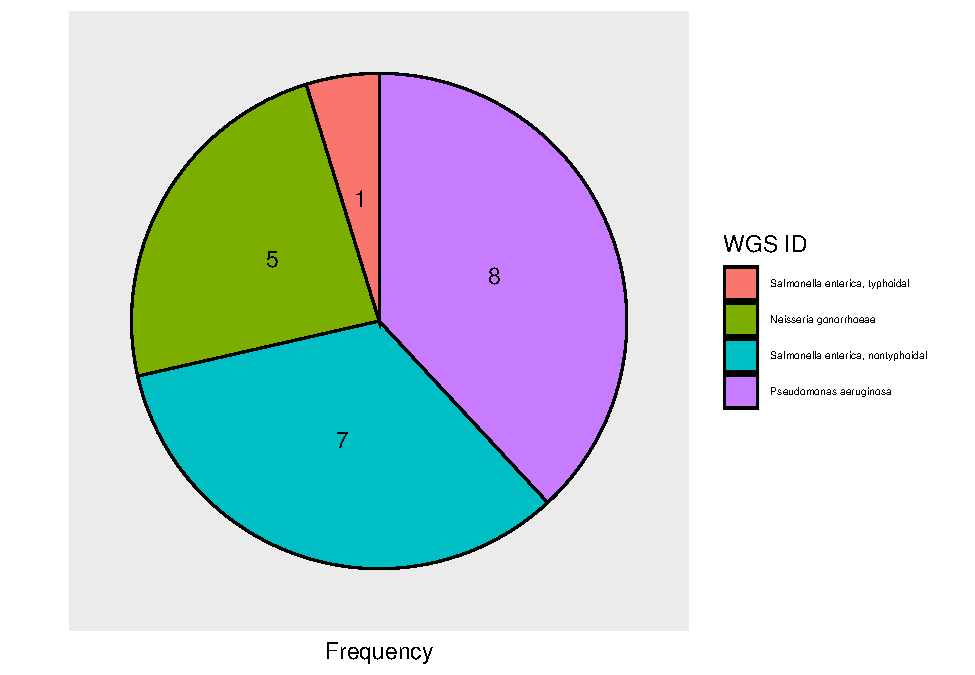
\includegraphics[keepaspectratio]{ARSRL_WGS_QC_report_2025-07-08_A_files/figure-latex/pie_chart-1.pdf}}

\subsubsection{Result Classification}\label{result-classification}

\pandocbounded{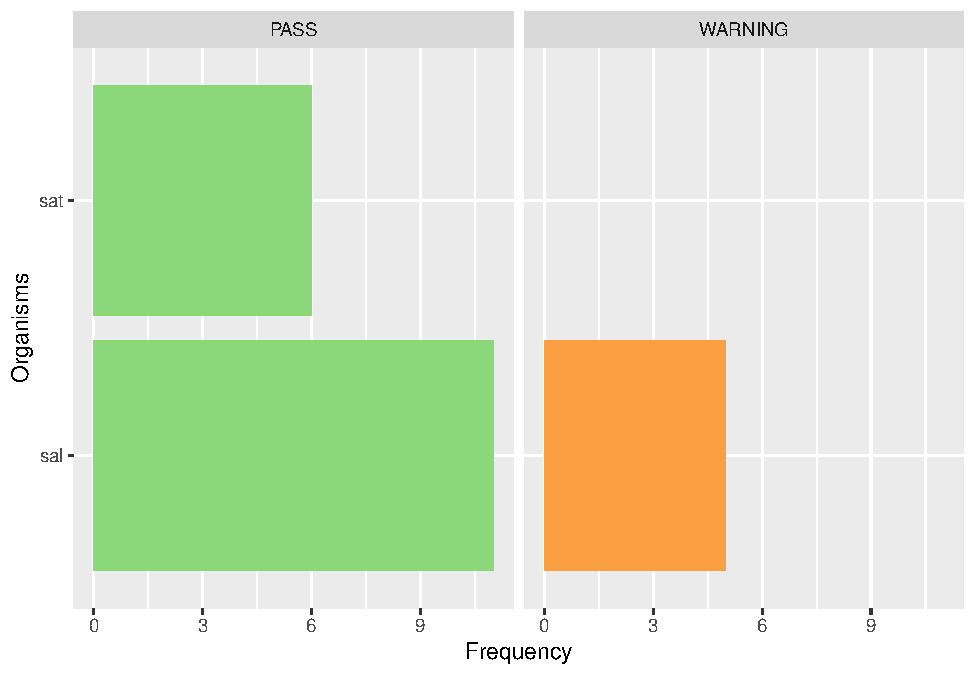
\includegraphics[keepaspectratio]{ARSRL_WGS_QC_report_2025-07-08_A_files/figure-latex/organism results-1.pdf}}

\subsubsection{Number of contigs}\label{number-of-contigs}

\pandocbounded{\includegraphics[keepaspectratio]{ARSRL_WGS_QC_report_2025-07-08_A_files/figure-latex/contigs_result-1.pdf}}

\subsubsection{N50 Value}\label{n50-value}

\pandocbounded{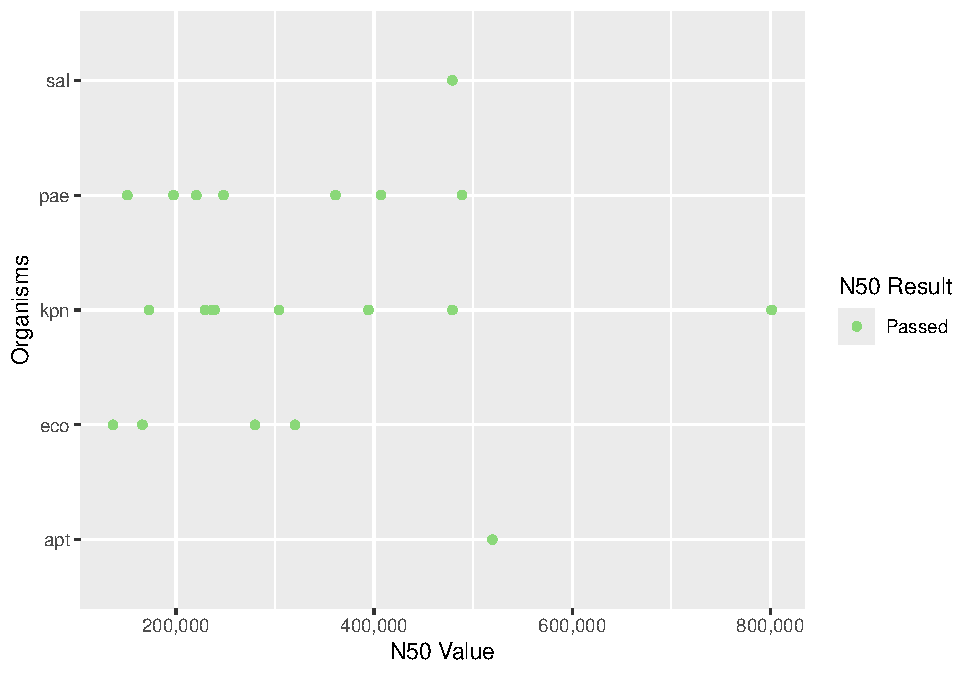
\includegraphics[keepaspectratio]{ARSRL_WGS_QC_report_2025-07-08_A_files/figure-latex/n50_result -1.pdf}}

\subsubsection{Total Length}\label{total-length}

\pandocbounded{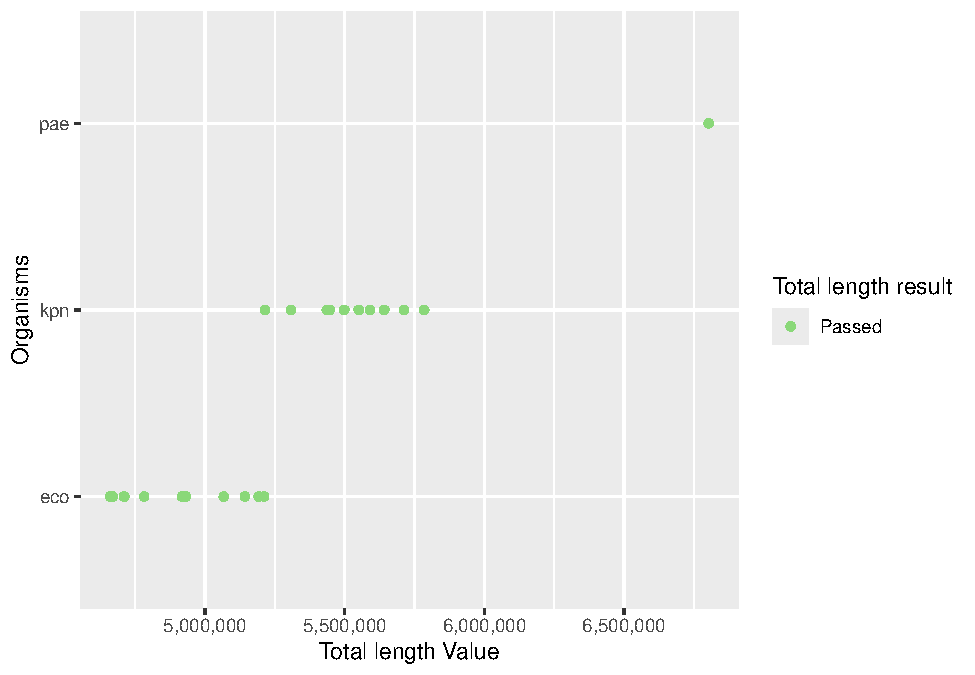
\includegraphics[keepaspectratio]{ARSRL_WGS_QC_report_2025-07-08_A_files/figure-latex/length_result -1.pdf}}

\fontsize{7}{8}
\selectfont
\captionsetup[table]{labelformat=empty}
\renewcommand{\arraystretch}{1}

\subsubsection{MLST RESULTS}\label{mlst-results}

\resizebox{\ifdim\width>\linewidth\linewidth\else\width\fi}{!}{
\begin{tabular}{>{\centering\arraybackslash}p{3cm}>{\centering\arraybackslash}p{3cm}>{\centering\arraybackslash}p{1cm}>{\centering\arraybackslash}p{1cm}>{\centering\arraybackslash}p{1cm}>{\centering\arraybackslash}p{1cm}>{\centering\arraybackslash}p{1cm}>{\centering\arraybackslash}p{1cm}>{\centering\arraybackslash}p{1cm}>{\centering\arraybackslash}p{1cm}}
\toprule
\cellcolor[HTML]{D4D4D4}{\textbf{sample\_id}} & \cellcolor[HTML]{D4D4D4}{\textbf{species}} & \cellcolor[HTML]{D4D4D4}{\textbf{MLST}} & \cellcolor[HTML]{D4D4D4}{\textbf{gapA}} & \cellcolor[HTML]{D4D4D4}{\textbf{infB}} & \cellcolor[HTML]{D4D4D4}{\textbf{mdh}} & \cellcolor[HTML]{D4D4D4}{\textbf{pgi}} & \cellcolor[HTML]{D4D4D4}{\textbf{phoE}} & \cellcolor[HTML]{D4D4D4}{\textbf{rpoB}} & \cellcolor[HTML]{D4D4D4}{\textbf{tonB}}\\
\midrule
25ARS\_CVM0028 & \em{Klebsiella pneumoniae} & 60 & 2 & 1 & 2 & 1 & 4 & 4 & 8\\
25ARS\_CVM0029 & \em{Klebsiella variicola} & - & \textasciitilde{}149 & 24 & 21 & 27 & 52 & 22 & 67\\
25ARS\_DMC0067 & \em{Klebsiella pneumoniae} & 15 & 1 & 1 & 1 & 1 & 1 & 1 & 1\\
25ARS\_EVR0022 & \em{Klebsiella pneumoniae} & 86 & 9 & 4 & 2 & 1 & 1 & 1 & 27\\
25ARS\_MMH0017 & \em{Klebsiella pneumoniae} & 278 & 4 & 1 & 1 & 1 & 12 & 1 & 4\\
\addlinespace
25ARS\_MMH0018 & \em{Klebsiella pneumoniae} & 268 & 2 & 1 & 2 & 1 & 7 & 1 & 81\\
25ARS\_NKI0015 & \em{Klebsiella pneumoniae} & 4845 & 2 & 1 & 62 & 3 & 10 & 4 & 4\\
25ARS\_NKI0016 & \em{Klebsiella pneumoniae} & 147 & 3 & 4 & 6 & 1 & 7 & 4 & 38\\
25ARS\_NMC0030 & \em{Klebsiella pneumoniae} & 2167 & 2 & 9 & 2 & 1 & 13 & 1 & 35\\
25ARS\_RMC0006 & \em{Klebsiella pneumoniae} & 515 & 2 & 1 & 1 & 1 & 1 & 1 & 4\\
\addlinespace
25ARS\_RMC0007 & \em{Klebsiella pneumoniae} & 515 & 2 & 1 & 1 & 1 & 1 & 1 & 4\\
25ARS\_RMC0010 & \em{Klebsiella pneumoniae} & 515 & 2 & 1 & 1 & 1 & 1 & 1 & 4\\
25ARS\_RMC0011 & \em{Klebsiella pneumoniae} & 515 & 2 & 1 & 1 & 1 & 1 & 1 & 4\\
25ARS\_STU0018 & \em{Klebsiella pneumoniae} & 307 & 4 & 1 & 2 & 52 & 1 & 1 & 7\\
25ARS\_ZMC0006 & \em{Klebsiella pneumoniae} & 37 & 2 & 9 & 2 & 1 & 13 & 1 & 16\\
\bottomrule
\multicolumn{10}{l}{\rule{0pt}{1em}\textit{Legend: } (-) Not identified}\\
\end{tabular}}

\resizebox{\ifdim\width>\linewidth\linewidth\else\width\fi}{!}{
\begin{tabular}{>{\centering\arraybackslash}p{3cm}>{\centering\arraybackslash}p{3cm}>{\centering\arraybackslash}p{1cm}>{\centering\arraybackslash}p{1cm}>{\centering\arraybackslash}p{1cm}>{\centering\arraybackslash}p{1cm}>{\centering\arraybackslash}p{1cm}>{\centering\arraybackslash}p{1cm}>{\centering\arraybackslash}p{1cm}>{\centering\arraybackslash}p{1cm}}
\toprule
\cellcolor[HTML]{D4D4D4}{\textbf{sample\_id}} & \cellcolor[HTML]{D4D4D4}{\textbf{species}} & \cellcolor[HTML]{D4D4D4}{\textbf{MLST}} & \cellcolor[HTML]{D4D4D4}{\textbf{gapA}} & \cellcolor[HTML]{D4D4D4}{\textbf{infB}} & \cellcolor[HTML]{D4D4D4}{\textbf{mdh}} & \cellcolor[HTML]{D4D4D4}{\textbf{pgi}} & \cellcolor[HTML]{D4D4D4}{\textbf{phoE}} & \cellcolor[HTML]{D4D4D4}{\textbf{rpoB}} & \cellcolor[HTML]{D4D4D4}{\textbf{tonB}}\\
\midrule
25ARS\_DMC0027 & \em{Escherichia coli} & - & 10 & 11 & 4 & 8 & 8 & 572 & 7\\
25ARS\_DMC0030 & \em{Escherichia coli} & 2083 & 6 & 322 & 5 & 16 & 11 & 8 & 7\\
25ARS\_NMC0006 & \em{Escherichia coli} & 361 & 10 & 99 & 5 & 91 & 8 & 7 & 2\\
25ARS\_NMC0007 & \em{Escherichia coli} & 361 & 10 & 99 & 5 & 91 & 8 & 7 & 2\\
UTPN\_BL\_018 & \em{Escherichia coli} & 12 & 13 & 13 & 9 & 13 & 16 & 10 & 9\\
\addlinespace
UTPN\_BL\_019 & \em{Escherichia coli} & 69 & 21 & 35 & 27 & 6 & 5 & 5 & 4\\
UTPR\_BL\_004 & \em{Escherichia coli} & 131 & 53 & 40 & 47 & 13 & 36 & 28 & 29\\
\bottomrule
\multicolumn{10}{l}{\rule{0pt}{1em}\textit{Legend: } (-) Not identified}\\
\end{tabular}}

\subsubsection{MLST RESULTS SUMMARY:}\label{mlst-results-summary}

\begin{tabular}{>{\raggedright\arraybackslash}p{6cm}>{\raggedright\arraybackslash}p{10cm}}
\toprule
\cellcolor[HTML]{D4D4D4}{\textbf{wgs\_id}} & \cellcolor[HTML]{D4D4D4}{\textbf{mlst\_count}}\\
\midrule
\em{Klebsiella pneumoniae} & 60 (n= 1 ), 15 (n= 1 ), 86 (n= 1 ), 278 (n= 1 ), 268 (n= 1 ), 4845 (n= 1 ), 147 (n= 1 ), 2167 (n= 1 ), 515 (n= 4 ), 307 (n= 1 ), 37 (n= 1 )\\
\em{Klebsiella variicola} & - (n= 1 )\\
\em{Escherichia coli} & - (n= 1 ), 2083 (n= 1 ), 361 (n= 2 ), 12 (n= 1 ), 69 (n= 1 ), 131 (n= 1 )\\
\bottomrule
\multicolumn{2}{l}{\rule{0pt}{1em}\textit{Legend: } (-) Not identified}\\
\end{tabular}

\newpage
\begin{landscape}
\fontsize{7}{8}
\selectfont
\captionsetup[table]{labelformat=empty}
\renewcommand{\arraystretch}{1.2}


\normalsize\textbf{AMR PREDICTION RESULTS}\textbf\normalsize




\fontsize{7}{8}
\selectfont
\captionsetup[table]{labelformat=empty}
\renewcommand{\arraystretch}{1.2}

\begingroup\fontsize{7}{9}\selectfont

\resizebox{\ifdim\width>\linewidth\linewidth\else\width\fi}{!}{
\begin{tabular}{c>{\centering\arraybackslash}p{3cm}>{\centering\arraybackslash}p{3cm}>{\centering\arraybackslash}p{3cm}>{\centering\arraybackslash}p{3cm}>{\centering\arraybackslash}p{3cm}>{\centering\arraybackslash}p{3cm}}
\toprule
\multicolumn{7}{l}{\textbf{\textit{Klebsiella pneumoniae} (Part 1.1)}} \\
\cmidrule(l{3pt}r{3pt}){1-7}
\cellcolor[HTML]{D4D4D4}{\textbf{sample\_id}} & \cellcolor[HTML]{D4D4D4}{\textbf{AMR AMIKACIN/ KAMYCIN/ QUINOLONE/ TOBRAMYCIN}} & \cellcolor[HTML]{D4D4D4}{\textbf{AMR AMINOGLYCOSIDE}} & \cellcolor[HTML]{D4D4D4}{\textbf{AMR AZITHROMYCIN/ ERYTHROMYCIN/ SPIRAMYCIN/ TELITHROMYCIN}} & \cellcolor[HTML]{D4D4D4}{\textbf{AMR BETA-LACTAM}} & \cellcolor[HTML]{D4D4D4}{\textbf{AMR BLEOMYCIN}} & \cellcolor[HTML]{D4D4D4}{\textbf{AMR CARBAPENEM}}\\
\midrule
25ARS\_CVM0028 & NA & NA & NA & blaSHV-11 & NA & NA\\
25ARS\_DMC0067 & NA & rmtC & NA & blaSHV-28 & ble & blaNDM-1\\
25ARS\_EVR0022 & NA & NA & NA & blaSHV-1 & NA & NA\\
25ARS\_MMH0017 & NA & NA & NA & blaSHV-27 & NA & NA\\
25ARS\_MMH0018 & NA & NA & NA & blaSHV-11 & NA & NA\\
\addlinespace
25ARS\_NKI0015 & NA & NA & mph(A) & blaTEM, blaTEM, blaSHV-76, blaOXA & NA & blaKPC-2\\
\bottomrule
\end{tabular}}
\endgroup{}


\vspace{5mm}

\begingroup\fontsize{7}{9}\selectfont

\resizebox{\ifdim\width>\linewidth\linewidth\else\width\fi}{!}{
\begin{tabular}{c>{\centering\arraybackslash}p{3cm}>{\centering\arraybackslash}p{3cm}>{\centering\arraybackslash}p{3cm}>{\centering\arraybackslash}p{3cm}>{\centering\arraybackslash}p{3cm}>{\centering\arraybackslash}p{3cm}}
\toprule
\multicolumn{7}{l}{\textbf{\textit{Klebsiella pneumoniae} (Part 1.2)}} \\
\cmidrule(l{3pt}r{3pt}){1-7}
\cellcolor[HTML]{D4D4D4}{\textbf{sample\_id}} & \cellcolor[HTML]{D4D4D4}{\textbf{AMR CEPHALOSPORIN}} & \cellcolor[HTML]{D4D4D4}{\textbf{AMR CHLORAMPHENICOL}} & \cellcolor[HTML]{D4D4D4}{\textbf{AMR CHLORAMPHENICOL/ FLORFENICOL}} & \cellcolor[HTML]{D4D4D4}{\textbf{AMR EFFLUX}} & \cellcolor[HTML]{D4D4D4}{\textbf{AMR FOSFOMYCIN}} & \cellcolor[HTML]{D4D4D4}{\textbf{AMR GENTAMICIN}}\\
\midrule
25ARS\_CVM0028 & NA & NA & NA & kdeA, emrD & fosA & NA\\
25ARS\_DMC0067 & NA & NA & NA & emrD, kdeA & fosA & NA\\
25ARS\_EVR0022 & NA & NA & NA & kdeA, emrD & fosA10 & NA\\
25ARS\_MMH0017 & NA & NA & NA & kdeA, emrD & fosA & NA\\
25ARS\_MMH0018 & NA & NA & NA & kdeA, emrD & fosA5 & NA\\
\addlinespace
25ARS\_NKI0015 & blaCTX-M-15 & NA & NA & kdeA, emrD & fosA, fosA7 & aac(3)-IId\\
\bottomrule
\end{tabular}}
\endgroup{}


\vspace{5mm}

\begingroup\fontsize{7}{9}\selectfont

\resizebox{\ifdim\width>\linewidth\linewidth\else\width\fi}{!}{
\begin{tabular}{c>{\centering\arraybackslash}p{3cm}>{\centering\arraybackslash}p{3cm}>{\centering\arraybackslash}p{3cm}>{\centering\arraybackslash}p{3cm}>{\centering\arraybackslash}p{3cm}>{\centering\arraybackslash}p{3cm}}
\toprule
\multicolumn{7}{l}{\textbf{\textit{Klebsiella pneumoniae} (Part 1.3)}} \\
\cmidrule(l{3pt}r{3pt}){1-7}
\cellcolor[HTML]{D4D4D4}{\textbf{sample\_id}} & \cellcolor[HTML]{D4D4D4}{\textbf{AMR KAMYCIN}} & \cellcolor[HTML]{D4D4D4}{\textbf{AMR PHENICOL/ QUINOLONE}} & \cellcolor[HTML]{D4D4D4}{\textbf{AMR QUINOLONE}} & \cellcolor[HTML]{D4D4D4}{\textbf{AMR RIFAMYCIN}} & \cellcolor[HTML]{D4D4D4}{\textbf{AMR STREPTOMYCIN}} & \cellcolor[HTML]{D4D4D4}{\textbf{AMR SULFOMIDE}}\\
\midrule
25ARS\_CVM0028 & NA & oqxA10, oqxB19 & NA & NA & NA & NA\\
25ARS\_DMC0067 & NA & oqxA, oqxB & NA & NA & NA & sul1\\
25ARS\_EVR0022 & NA & oqxA11, oqxB19 & NA & NA & NA & NA\\
25ARS\_MMH0017 & NA & oqxB, oqxA & NA & NA & NA & NA\\
25ARS\_MMH0018 & NA & oqxA, oqxB5 & NA & NA & NA & NA\\
\addlinespace
25ARS\_NKI0015 & NA & oqxA, oqxB & qnrS1 & NA & aph(3'')-Ib, aph(6)-Id & sul2\\
\bottomrule
\end{tabular}}
\endgroup{}


\vspace{5mm}

\begingroup\fontsize{7}{9}\selectfont

\resizebox{\ifdim\width>\linewidth\linewidth\else\width\fi}{!}{
\begin{tabular}{c>{\centering\arraybackslash}p{3cm}>{\centering\arraybackslash}p{3cm}>{\centering\arraybackslash}p{3cm}>{\centering\arraybackslash}p{3cm}>{\centering\arraybackslash}p{3cm}>{\centering\arraybackslash}p{3cm}}
\toprule
\multicolumn{7}{l}{\textbf{\textit{Klebsiella pneumoniae} (Part 1.4)}} \\
\cmidrule(l{3pt}r{3pt}){1-7}
\cellcolor[HTML]{D4D4D4}{\textbf{sample\_id}} & \cellcolor[HTML]{D4D4D4}{\textbf{AMR TETRACYCLINE}} & \cellcolor[HTML]{D4D4D4}{\textbf{AMR TRIMETHOPRIM}} & \cellcolor[HTML]{D4D4D4}{\textbf{STRESS }} & \cellcolor[HTML]{D4D4D4}{\textbf{STRESS ARSENIC}} & \cellcolor[HTML]{D4D4D4}{\textbf{STRESS ARSENITE}} & \cellcolor[HTML]{D4D4D4}{\textbf{STRESS ARSETE}}\\
\midrule
25ARS\_CVM0028 & NA & NA & fieF, asr & NA & NA & arsC\\
25ARS\_DMC0067 & NA & NA & fieF, asr & NA & NA & arsC\\
25ARS\_EVR0022 & NA & NA & fieF, asr & NA & NA & arsC\\
25ARS\_MMH0017 & NA & NA & fieF, asr & arsR, arsR & arsD, arsB, arsA, arsD & arsC, arsC, arsC, arsC\\
25ARS\_MMH0018 & NA & NA & fieF & NA & NA & arsC\\
\addlinespace
25ARS\_NKI0015 & NA & NA & fieF, asr & arsR & arsD & arsC\\
\bottomrule
\end{tabular}}
\endgroup{}


\vspace{5mm}

\begingroup\fontsize{7}{9}\selectfont

\resizebox{\ifdim\width>\linewidth\linewidth\else\width\fi}{!}{
\begin{tabular}{c>{\centering\arraybackslash}p{3cm}>{\centering\arraybackslash}p{3cm}>{\centering\arraybackslash}p{3cm}>{\centering\arraybackslash}p{3cm}>{\centering\arraybackslash}p{3cm}>{\centering\arraybackslash}p{3cm}}
\toprule
\multicolumn{7}{l}{\textbf{\textit{Klebsiella pneumoniae} (Part 1.5)}} \\
\cmidrule(l{3pt}r{3pt}){1-7}
\cellcolor[HTML]{D4D4D4}{\textbf{sample\_id}} & \cellcolor[HTML]{D4D4D4}{\textbf{STRESS COPPER}} & \cellcolor[HTML]{D4D4D4}{\textbf{STRESS COPPER/ SILVER}} & \cellcolor[HTML]{D4D4D4}{\textbf{STRESS FLUORIDE}} & \cellcolor[HTML]{D4D4D4}{\textbf{STRESS MERCURY}} & \cellcolor[HTML]{D4D4D4}{\textbf{STRESS ORGANOMERCURY}} & \cellcolor[HTML]{D4D4D4}{\textbf{STRESS QUATERRY AMMONIUM}}\\
\midrule
25ARS\_CVM0028 & NA & NA & NA & NA & NA & NA\\
25ARS\_DMC0067 & NA & NA & NA & NA & NA & NA\\
25ARS\_EVR0022 & pcoS, pcoR, pcoD, pcoC, pcoB, pcoA & silA, silB, silF, silC, silR, silS & crcB & NA & NA & NA\\
25ARS\_MMH0017 & NA & silA & NA & NA & NA & NA\\
25ARS\_MMH0018 & pcoA, pcoB, pcoC, pcoD, pcoR, pcoS & silC, silS, silR, silF, silB, silA & NA & NA & NA & NA\\
\addlinespace
25ARS\_NKI0015 & NA & NA & NA & merA, merD, merE & merC & NA\\
\bottomrule
\end{tabular}}
\endgroup{}


\vspace{5mm}

\begingroup\fontsize{7}{9}\selectfont

\resizebox{\ifdim\width>\linewidth\linewidth\else\width\fi}{!}{
\begin{tabular}{c>{\centering\arraybackslash}p{3cm}>{\centering\arraybackslash}p{3cm}>{\centering\arraybackslash}p{3cm}}
\toprule
\multicolumn{4}{l}{\textbf{\textit{Klebsiella pneumoniae} (Part 1.6)}} \\
\cmidrule(l{3pt}r{3pt}){1-4}
\cellcolor[HTML]{D4D4D4}{\textbf{sample\_id}} & \cellcolor[HTML]{D4D4D4}{\textbf{STRESS SILVER}} & \cellcolor[HTML]{D4D4D4}{\textbf{STRESS TELLURIUM}} & \cellcolor[HTML]{D4D4D4}{\textbf{VIRULENCE }}\\
\midrule
25ARS\_CVM0028 & NA & NA & ybtQ, ybtP, iroN, iroB, iroC, iroD, rmpC, rmpD, rmpA\\
25ARS\_DMC0067 & NA & NA & ybtP, ybtQ\\
25ARS\_EVR0022 & silP & terE, terD, terC, terB & iroB, ybtQ, ybtP, rmpA2, iutA, iucC, iucB, iucA, iroN, peg-344, iroC, iroD, rmpA, rmpC, rmpD\\
25ARS\_MMH0017 & NA & NA & NA\\
25ARS\_MMH0018 & silP & terC, terB, terE, terD & iucA, iucB, iucC, iutA, rmpA2, ybtP, ybtQ, rmpA, rmpD, rmpC, peg-344, iroN, iroD, iroC, iroB\\
\addlinespace
25ARS\_NKI0015 & NA & NA & NA\\
\bottomrule
\end{tabular}}
\endgroup{}


\vspace{10mm}

\begingroup\fontsize{7}{9}\selectfont

\resizebox{\ifdim\width>\linewidth\linewidth\else\width\fi}{!}{
\begin{tabular}{l>{\centering\arraybackslash}p{3cm}>{\centering\arraybackslash}p{3cm}>{\centering\arraybackslash}p{3cm}>{\centering\arraybackslash}p{3cm}>{\centering\arraybackslash}p{3cm}>{\centering\arraybackslash}p{3cm}c}
\toprule
\multicolumn{7}{l}{\textbf{\textit{Klebsiella pneumoniae} (Part 2.1)}} \\
\cmidrule(l{3pt}r{3pt}){1-7}
\cellcolor[HTML]{D4D4D4}{\textbf{ }} & \cellcolor[HTML]{D4D4D4}{\textbf{sample\_id}} & \cellcolor[HTML]{D4D4D4}{\textbf{AMR AMIKACIN/ KAMYCIN/ QUINOLONE/ TOBRAMYCIN}} & \cellcolor[HTML]{D4D4D4}{\textbf{AMR AMINOGLYCOSIDE}} & \cellcolor[HTML]{D4D4D4}{\textbf{AMR AZITHROMYCIN/ ERYTHROMYCIN/ SPIRAMYCIN/ TELITHROMYCIN}} & \cellcolor[HTML]{D4D4D4}{\textbf{AMR BETA-LACTAM}} & \cellcolor[HTML]{D4D4D4}{\textbf{AMR BLEOMYCIN}} & \cellcolor[HTML]{D4D4D4}{\textbf{AMR CARBAPENEM}}\\
\midrule
7 & 25ARS\_NKI0016 & NA & NA & mph(A) & blaSHV-11, blaOXA, blaTEM-1 & NA & blaKPC-2\\
8 & 25ARS\_NMC0030 & aac(6')-Ib-cr5 & NA & mph(A) & blaTEM-1, blaSHV-11 & NA & NA\\
9 & 25ARS\_RMC0006 & aac(6')-Ib-cr5 & rmtC & mph(A) & blaSHV-1, blaTEM & ble & blaNDM-1\\
10 & 25ARS\_RMC0007 & aac(6')-Ib-cr5 & rmtC & mph(A) & blaTEM, blaSHV-1 & ble & blaNDM-1\\
11 & 25ARS\_RMC0010 & aac(6')-Ib-cr5 & rmtC & mph(A) & blaTEM, blaSHV-1 & ble & blaNDM-1\\
\addlinespace
12 & 25ARS\_RMC0011 & aac(6')-Ib-cr5 & rmtC & mph(A) & blaSHV-1, blaTEM-1 & ble & blaNDM-1\\
\bottomrule
\end{tabular}}
\endgroup{}


\vspace{5mm}

\begingroup\fontsize{7}{9}\selectfont

\resizebox{\ifdim\width>\linewidth\linewidth\else\width\fi}{!}{
\begin{tabular}{l>{\centering\arraybackslash}p{3cm}>{\centering\arraybackslash}p{3cm}>{\centering\arraybackslash}p{3cm}>{\centering\arraybackslash}p{3cm}>{\centering\arraybackslash}p{3cm}>{\centering\arraybackslash}p{3cm}c}
\toprule
\multicolumn{7}{l}{\textbf{\textit{Klebsiella pneumoniae} (Part 2.2)}} \\
\cmidrule(l{3pt}r{3pt}){1-7}
\cellcolor[HTML]{D4D4D4}{\textbf{ }} & \cellcolor[HTML]{D4D4D4}{\textbf{sample\_id}} & \cellcolor[HTML]{D4D4D4}{\textbf{AMR CEPHALOSPORIN}} & \cellcolor[HTML]{D4D4D4}{\textbf{AMR CHLORAMPHENICOL}} & \cellcolor[HTML]{D4D4D4}{\textbf{AMR CHLORAMPHENICOL/ FLORFENICOL}} & \cellcolor[HTML]{D4D4D4}{\textbf{AMR EFFLUX}} & \cellcolor[HTML]{D4D4D4}{\textbf{AMR FOSFOMYCIN}} & \cellcolor[HTML]{D4D4D4}{\textbf{AMR GENTAMICIN}}\\
\midrule
7 & 25ARS\_NKI0016 & NA & NA & NA & emrD, kdeA & fosA & aac(3)-IId\\
8 & 25ARS\_NMC0030 & blaCTX-M-15, blaOXA-1 & catB3 & NA & emrD, kdeA & fosA & aac(3)-IIe\\
9 & 25ARS\_RMC0006 & blaCTX-M & NA & floR & emrD, kdeA & fosA & aac(3)-IId\\
10 & 25ARS\_RMC0007 & blaCTX-M-15 & NA & floR & kdeA, emrD & fosA & aac(3)-IId\\
11 & 25ARS\_RMC0010 & blaCTX-M & NA & floR & kdeA, emrD & fosA & aac(3)-IId\\
\addlinespace
12 & 25ARS\_RMC0011 & blaCTX-M-15 & NA & floR & emrD, kdeA & fosA & aac(3)-IId\\
\bottomrule
\end{tabular}}
\endgroup{}


\vspace{5mm}

\begingroup\fontsize{7}{9}\selectfont

\resizebox{\ifdim\width>\linewidth\linewidth\else\width\fi}{!}{
\begin{tabular}{l>{\centering\arraybackslash}p{3cm}>{\centering\arraybackslash}p{3cm}>{\centering\arraybackslash}p{3cm}>{\centering\arraybackslash}p{3cm}>{\centering\arraybackslash}p{3cm}>{\centering\arraybackslash}p{3cm}c}
\toprule
\multicolumn{7}{l}{\textbf{\textit{Klebsiella pneumoniae} (Part 2.3)}} \\
\cmidrule(l{3pt}r{3pt}){1-7}
\cellcolor[HTML]{D4D4D4}{\textbf{ }} & \cellcolor[HTML]{D4D4D4}{\textbf{sample\_id}} & \cellcolor[HTML]{D4D4D4}{\textbf{AMR KAMYCIN}} & \cellcolor[HTML]{D4D4D4}{\textbf{AMR PHENICOL/ QUINOLONE}} & \cellcolor[HTML]{D4D4D4}{\textbf{AMR QUINOLONE}} & \cellcolor[HTML]{D4D4D4}{\textbf{AMR RIFAMYCIN}} & \cellcolor[HTML]{D4D4D4}{\textbf{AMR STREPTOMYCIN}} & \cellcolor[HTML]{D4D4D4}{\textbf{AMR SULFOMIDE}}\\
\midrule
7 & 25ARS\_NKI0016 & aph(3')-Ia & oqxB, oqxA & qnrB2 & NA & aadA2 & sul1\\
8 & 25ARS\_NMC0030 & NA & oqxA, oqxB & qnrB6 & arr-3 & aadA16 & sul1, sul1\\
9 & 25ARS\_RMC0006 & NA & oqxA, oqxB32 & qnrS1 & arr-3 & aadA16, aph(3'')-Ib, aph(6)-Id & sul2, sul1\\
10 & 25ARS\_RMC0007 & NA & oqxB32, oqxA & qnrS1 & arr-3 & aadA16, aph(3'')-Ib, aph(6)-Id & sul1, sul2\\
11 & 25ARS\_RMC0010 & NA & oqxA, oqxB32 & qnrS1 & arr-3 & aadA16, aph(6)-Id, aph(3'')-Ib & sul1, sul2\\
\addlinespace
12 & 25ARS\_RMC0011 & NA & oqxA, oqxB32 & qnrS1 & arr-3 & aadA16, aph(6)-Id, aph(3'')-Ib & sul1, sul2\\
\bottomrule
\end{tabular}}
\endgroup{}


\vspace{5mm}

\begingroup\fontsize{7}{9}\selectfont

\resizebox{\ifdim\width>\linewidth\linewidth\else\width\fi}{!}{
\begin{tabular}{l>{\centering\arraybackslash}p{3cm}>{\centering\arraybackslash}p{3cm}>{\centering\arraybackslash}p{3cm}>{\centering\arraybackslash}p{3cm}>{\centering\arraybackslash}p{3cm}>{\centering\arraybackslash}p{3cm}c}
\toprule
\multicolumn{7}{l}{\textbf{\textit{Klebsiella pneumoniae} (Part 2.4)}} \\
\cmidrule(l{3pt}r{3pt}){1-7}
\cellcolor[HTML]{D4D4D4}{\textbf{ }} & \cellcolor[HTML]{D4D4D4}{\textbf{sample\_id}} & \cellcolor[HTML]{D4D4D4}{\textbf{AMR TETRACYCLINE}} & \cellcolor[HTML]{D4D4D4}{\textbf{AMR TRIMETHOPRIM}} & \cellcolor[HTML]{D4D4D4}{\textbf{STRESS }} & \cellcolor[HTML]{D4D4D4}{\textbf{STRESS ARSENIC}} & \cellcolor[HTML]{D4D4D4}{\textbf{STRESS ARSENITE}} & \cellcolor[HTML]{D4D4D4}{\textbf{STRESS ARSETE}}\\
\midrule
7 & 25ARS\_NKI0016 & NA & dfrA12 & fieF & NA & NA & arsC, arsC\\
8 & 25ARS\_NMC0030 & tet(A) & dfrA27 & fieF, clpK, hsp20 & NA & NA & arsC\\
9 & 25ARS\_RMC0006 & tet(A) & dfrA27 & fieF, hsp20, clpK & NA & NA & arsC\\
10 & 25ARS\_RMC0007 & tet(A) & dfrA27 & fieF, clpK, hsp20 & NA & NA & arsC\\
11 & 25ARS\_RMC0010 & tet(A) & dfrA27 & fieF, hsp20, clpK & NA & NA & arsC\\
\addlinespace
12 & 25ARS\_RMC0011 & tet(A) & dfrA27 & hsp20, clpK, fieF & NA & NA & arsC\\
\bottomrule
\end{tabular}}
\endgroup{}


\vspace{5mm}

\begingroup\fontsize{7}{9}\selectfont

\resizebox{\ifdim\width>\linewidth\linewidth\else\width\fi}{!}{
\begin{tabular}{l>{\centering\arraybackslash}p{3cm}>{\centering\arraybackslash}p{3cm}>{\centering\arraybackslash}p{3cm}>{\centering\arraybackslash}p{3cm}>{\centering\arraybackslash}p{3cm}>{\centering\arraybackslash}p{3cm}c}
\toprule
\multicolumn{7}{l}{\textbf{\textit{Klebsiella pneumoniae} (Part 2.5)}} \\
\cmidrule(l{3pt}r{3pt}){1-7}
\cellcolor[HTML]{D4D4D4}{\textbf{ }} & \cellcolor[HTML]{D4D4D4}{\textbf{sample\_id}} & \cellcolor[HTML]{D4D4D4}{\textbf{STRESS COPPER}} & \cellcolor[HTML]{D4D4D4}{\textbf{STRESS COPPER/ SILVER}} & \cellcolor[HTML]{D4D4D4}{\textbf{STRESS FLUORIDE}} & \cellcolor[HTML]{D4D4D4}{\textbf{STRESS MERCURY}} & \cellcolor[HTML]{D4D4D4}{\textbf{STRESS ORGANOMERCURY}} & \cellcolor[HTML]{D4D4D4}{\textbf{STRESS QUATERRY AMMONIUM}}\\
\midrule
7 & 25ARS\_NKI0016 & NA & NA & NA & merA, merD, merE & merC & qacE\\
8 & 25ARS\_NMC0030 & pcoE, pcoR, pcoD, pcoC, pcoB, pcoA, pcoS & silA, silB, silF, silC, silR, silS & NA & NA & NA & qacEdelta1, qacEdelta1\\
9 & 25ARS\_RMC0006 & pcoE, pcoS, pcoR, pcoD, pcoC, pcoB, pcoA & silA, silB, silF, silC, silR, silS & NA & NA & NA & qacEdelta1\\
10 & 25ARS\_RMC0007 & pcoA, pcoB, pcoC, pcoD, pcoR, pcoS, pcoE & silS, silR, silC, silF, silB, silA & NA & NA & NA & qacEdelta1\\
11 & 25ARS\_RMC0010 & pcoA, pcoB, pcoC, pcoD, pcoR, pcoS, pcoE & silA, silB, silF, silC, silR, silS & NA & NA & NA & qacEdelta1\\
\addlinespace
12 & 25ARS\_RMC0011 & pcoC, pcoA, pcoB, pcoD, pcoR, pcoS, pcoE & silS, silR, silC, silF, silB, silA & NA & NA & NA & NA\\
\bottomrule
\end{tabular}}
\endgroup{}


\vspace{5mm}

\begingroup\fontsize{7}{9}\selectfont

\resizebox{\ifdim\width>\linewidth\linewidth\else\width\fi}{!}{
\begin{tabular}{l>{\centering\arraybackslash}p{3cm}>{\centering\arraybackslash}p{3cm}>{\centering\arraybackslash}p{3cm}c}
\toprule
\multicolumn{4}{l}{\textbf{\textit{Klebsiella pneumoniae} (Part 2.6)}} \\
\cmidrule(l{3pt}r{3pt}){1-4}
\cellcolor[HTML]{D4D4D4}{\textbf{ }} & \cellcolor[HTML]{D4D4D4}{\textbf{sample\_id}} & \cellcolor[HTML]{D4D4D4}{\textbf{STRESS SILVER}} & \cellcolor[HTML]{D4D4D4}{\textbf{STRESS TELLURIUM}} & \cellcolor[HTML]{D4D4D4}{\textbf{VIRULENCE }}\\
\midrule
7 & 25ARS\_NKI0016 & NA & NA & ybtQ, ybtP\\
8 & 25ARS\_NMC0030 & silP, silE & NA & NA\\
9 & 25ARS\_RMC0006 & silP, silE & NA & ybtP, ybtQ\\
10 & 25ARS\_RMC0007 & silE, silP & NA & ybtQ, ybtP\\
11 & 25ARS\_RMC0010 & silP, silE & NA & ybtQ, ybtP\\
\addlinespace
12 & 25ARS\_RMC0011 & silE, silP & NA & ybtP, ybtQ\\
\bottomrule
\end{tabular}}
\endgroup{}


\vspace{10mm}

\begingroup\fontsize{7}{9}\selectfont

\resizebox{\ifdim\width>\linewidth\linewidth\else\width\fi}{!}{
\begin{tabular}{l>{\centering\arraybackslash}p{3cm}>{\centering\arraybackslash}p{3cm}>{\centering\arraybackslash}p{3cm}>{\centering\arraybackslash}p{3cm}>{\centering\arraybackslash}p{3cm}>{\centering\arraybackslash}p{3cm}c}
\toprule
\multicolumn{7}{l}{\textbf{\textit{Klebsiella pneumoniae} (Part 3.1)}} \\
\cmidrule(l{3pt}r{3pt}){1-7}
\cellcolor[HTML]{D4D4D4}{\textbf{ }} & \cellcolor[HTML]{D4D4D4}{\textbf{sample\_id}} & \cellcolor[HTML]{D4D4D4}{\textbf{AMR AMIKACIN/ KAMYCIN/ QUINOLONE/ TOBRAMYCIN}} & \cellcolor[HTML]{D4D4D4}{\textbf{AMR AMINOGLYCOSIDE}} & \cellcolor[HTML]{D4D4D4}{\textbf{AMR AZITHROMYCIN/ ERYTHROMYCIN/ SPIRAMYCIN/ TELITHROMYCIN}} & \cellcolor[HTML]{D4D4D4}{\textbf{AMR BETA-LACTAM}} & \cellcolor[HTML]{D4D4D4}{\textbf{AMR BLEOMYCIN}} & \cellcolor[HTML]{D4D4D4}{\textbf{AMR CARBAPENEM}}\\
\midrule
13 & 25ARS\_STU0018 & aac(6')-Ib-cr5 & NA & NA & blaSHV-28, blaTEM-1 & NA & NA\\
14 & 25ARS\_ZMC0006 & NA & NA & NA & blaSHV-11 & NA & NA\\
\bottomrule
\end{tabular}}
\endgroup{}


\vspace{5mm}

\begingroup\fontsize{7}{9}\selectfont

\resizebox{\ifdim\width>\linewidth\linewidth\else\width\fi}{!}{
\begin{tabular}{l>{\centering\arraybackslash}p{3cm}>{\centering\arraybackslash}p{3cm}>{\centering\arraybackslash}p{3cm}>{\centering\arraybackslash}p{3cm}>{\centering\arraybackslash}p{3cm}>{\centering\arraybackslash}p{3cm}c}
\toprule
\multicolumn{7}{l}{\textbf{\textit{Klebsiella pneumoniae} (Part 3.2)}} \\
\cmidrule(l{3pt}r{3pt}){1-7}
\cellcolor[HTML]{D4D4D4}{\textbf{ }} & \cellcolor[HTML]{D4D4D4}{\textbf{sample\_id}} & \cellcolor[HTML]{D4D4D4}{\textbf{AMR CEPHALOSPORIN}} & \cellcolor[HTML]{D4D4D4}{\textbf{AMR CHLORAMPHENICOL}} & \cellcolor[HTML]{D4D4D4}{\textbf{AMR CHLORAMPHENICOL/ FLORFENICOL}} & \cellcolor[HTML]{D4D4D4}{\textbf{AMR EFFLUX}} & \cellcolor[HTML]{D4D4D4}{\textbf{AMR FOSFOMYCIN}} & \cellcolor[HTML]{D4D4D4}{\textbf{AMR GENTAMICIN}}\\
\midrule
13 & 25ARS\_STU0018 & blaCTX-M-15, blaOXA-1 & catB3 & NA & emrD, kdeA & fosA & NA\\
14 & 25ARS\_ZMC0006 & NA & NA & NA & kdeA, emrD & fosA & NA\\
\bottomrule
\end{tabular}}
\endgroup{}


\vspace{5mm}

\begingroup\fontsize{7}{9}\selectfont

\resizebox{\ifdim\width>\linewidth\linewidth\else\width\fi}{!}{
\begin{tabular}{l>{\centering\arraybackslash}p{3cm}>{\centering\arraybackslash}p{3cm}>{\centering\arraybackslash}p{3cm}>{\centering\arraybackslash}p{3cm}>{\centering\arraybackslash}p{3cm}>{\centering\arraybackslash}p{3cm}c}
\toprule
\multicolumn{7}{l}{\textbf{\textit{Klebsiella pneumoniae} (Part 3.3)}} \\
\cmidrule(l{3pt}r{3pt}){1-7}
\cellcolor[HTML]{D4D4D4}{\textbf{ }} & \cellcolor[HTML]{D4D4D4}{\textbf{sample\_id}} & \cellcolor[HTML]{D4D4D4}{\textbf{AMR KAMYCIN}} & \cellcolor[HTML]{D4D4D4}{\textbf{AMR PHENICOL/ QUINOLONE}} & \cellcolor[HTML]{D4D4D4}{\textbf{AMR QUINOLONE}} & \cellcolor[HTML]{D4D4D4}{\textbf{AMR RIFAMYCIN}} & \cellcolor[HTML]{D4D4D4}{\textbf{AMR STREPTOMYCIN}} & \cellcolor[HTML]{D4D4D4}{\textbf{AMR SULFOMIDE}}\\
\midrule
13 & 25ARS\_STU0018 & NA & oqxB19, oqxA & qnrB1 & NA & aph(3'')-Ib, aph(6)-Id & sul2\\
14 & 25ARS\_ZMC0006 & NA & oqxB, oqxA & NA & NA & NA & NA\\
\bottomrule
\end{tabular}}
\endgroup{}


\vspace{5mm}

\begingroup\fontsize{7}{9}\selectfont

\resizebox{\ifdim\width>\linewidth\linewidth\else\width\fi}{!}{
\begin{tabular}{l>{\centering\arraybackslash}p{3cm}>{\centering\arraybackslash}p{3cm}>{\centering\arraybackslash}p{3cm}>{\centering\arraybackslash}p{3cm}>{\centering\arraybackslash}p{3cm}>{\centering\arraybackslash}p{3cm}c}
\toprule
\multicolumn{7}{l}{\textbf{\textit{Klebsiella pneumoniae} (Part 3.4)}} \\
\cmidrule(l{3pt}r{3pt}){1-7}
\cellcolor[HTML]{D4D4D4}{\textbf{ }} & \cellcolor[HTML]{D4D4D4}{\textbf{sample\_id}} & \cellcolor[HTML]{D4D4D4}{\textbf{AMR TETRACYCLINE}} & \cellcolor[HTML]{D4D4D4}{\textbf{AMR TRIMETHOPRIM}} & \cellcolor[HTML]{D4D4D4}{\textbf{STRESS }} & \cellcolor[HTML]{D4D4D4}{\textbf{STRESS ARSENIC}} & \cellcolor[HTML]{D4D4D4}{\textbf{STRESS ARSENITE}} & \cellcolor[HTML]{D4D4D4}{\textbf{STRESS ARSETE}}\\
\midrule
13 & 25ARS\_STU0018 & tet(A) & dfrA14 & fieF, hsp20, clpK & arsR & arsD, arsA, arsB & arsC, arsC\\
14 & 25ARS\_ZMC0006 & NA & NA & fieF & NA & NA & arsC\\
\bottomrule
\end{tabular}}
\endgroup{}


\vspace{5mm}

\begingroup\fontsize{7}{9}\selectfont

\resizebox{\ifdim\width>\linewidth\linewidth\else\width\fi}{!}{
\begin{tabular}{l>{\centering\arraybackslash}p{3cm}>{\centering\arraybackslash}p{3cm}>{\centering\arraybackslash}p{3cm}>{\centering\arraybackslash}p{3cm}>{\centering\arraybackslash}p{3cm}>{\centering\arraybackslash}p{3cm}c}
\toprule
\multicolumn{7}{l}{\textbf{\textit{Klebsiella pneumoniae} (Part 3.5)}} \\
\cmidrule(l{3pt}r{3pt}){1-7}
\cellcolor[HTML]{D4D4D4}{\textbf{ }} & \cellcolor[HTML]{D4D4D4}{\textbf{sample\_id}} & \cellcolor[HTML]{D4D4D4}{\textbf{STRESS COPPER}} & \cellcolor[HTML]{D4D4D4}{\textbf{STRESS COPPER/ SILVER}} & \cellcolor[HTML]{D4D4D4}{\textbf{STRESS FLUORIDE}} & \cellcolor[HTML]{D4D4D4}{\textbf{STRESS MERCURY}} & \cellcolor[HTML]{D4D4D4}{\textbf{STRESS ORGANOMERCURY}} & \cellcolor[HTML]{D4D4D4}{\textbf{STRESS QUATERRY AMMONIUM}}\\
\midrule
13 & 25ARS\_STU0018 & pcoE, pcoS, pcoR, pcoD, pcoC, pcoB, pcoA & silA, silB, silF, silC, silR, silS & NA & NA & NA & NA\\
14 & 25ARS\_ZMC0006 & NA & NA & NA & NA & NA & NA\\
\bottomrule
\end{tabular}}
\endgroup{}


\vspace{5mm}

\begingroup\fontsize{7}{9}\selectfont

\resizebox{\ifdim\width>\linewidth\linewidth\else\width\fi}{!}{
\begin{tabular}{l>{\centering\arraybackslash}p{3cm}>{\centering\arraybackslash}p{3cm}>{\centering\arraybackslash}p{3cm}c}
\toprule
\multicolumn{4}{l}{\textbf{\textit{Klebsiella pneumoniae} (Part 3.6)}} \\
\cmidrule(l{3pt}r{3pt}){1-4}
\cellcolor[HTML]{D4D4D4}{\textbf{ }} & \cellcolor[HTML]{D4D4D4}{\textbf{sample\_id}} & \cellcolor[HTML]{D4D4D4}{\textbf{STRESS SILVER}} & \cellcolor[HTML]{D4D4D4}{\textbf{STRESS TELLURIUM}} & \cellcolor[HTML]{D4D4D4}{\textbf{VIRULENCE }}\\
\midrule
13 & 25ARS\_STU0018 & silP, silE & terB, terC, terD, terE & NA\\
14 & 25ARS\_ZMC0006 & NA & NA & NA\\
\bottomrule
\end{tabular}}
\endgroup{}
\begingroup\fontsize{7}{9}\selectfont

\resizebox{\ifdim\width>\linewidth\linewidth\else\width\fi}{!}{
\begin{tabular}{c>{\centering\arraybackslash}p{3cm}>{\centering\arraybackslash}p{3cm}>{\centering\arraybackslash}p{3cm}>{\centering\arraybackslash}p{3cm}>{\centering\arraybackslash}p{3cm}>{\centering\arraybackslash}p{3cm}}
\toprule
\multicolumn{7}{l}{\textbf{\textit{Klebsiella variicola} (Part 1.1)}} \\
\cmidrule(l{3pt}r{3pt}){1-7}
\cellcolor[HTML]{D4D4D4}{\textbf{sample\_id}} & \cellcolor[HTML]{D4D4D4}{\textbf{AMR BETA-LACTAM}} & \cellcolor[HTML]{D4D4D4}{\textbf{AMR EFFLUX}} & \cellcolor[HTML]{D4D4D4}{\textbf{AMR FOSFOMYCIN}} & \cellcolor[HTML]{D4D4D4}{\textbf{AMR PHENICOL/ QUINOLONE}} & \cellcolor[HTML]{D4D4D4}{\textbf{STRESS }} & \cellcolor[HTML]{D4D4D4}{\textbf{STRESS ARSETE}}\\
\midrule
25ARS\_CVM0029 & blaLEN-7 & emrD, kdeA & fosA & oqxB, oqxA & fieF & arsC\\
\bottomrule
\end{tabular}}
\endgroup{}
\begingroup\fontsize{7}{9}\selectfont

\resizebox{\ifdim\width>\linewidth\linewidth\else\width\fi}{!}{
\begin{tabular}{c>{\centering\arraybackslash}p{3cm}>{\centering\arraybackslash}p{3cm}>{\centering\arraybackslash}p{3cm}>{\centering\arraybackslash}p{3cm}>{\centering\arraybackslash}p{3cm}>{\centering\arraybackslash}p{3cm}}
\toprule
\multicolumn{7}{l}{\textbf{\textit{Escherichia coli} (Part 1.1)}} \\
\cmidrule(l{3pt}r{3pt}){1-7}
\cellcolor[HTML]{D4D4D4}{\textbf{sample\_id}} & \cellcolor[HTML]{D4D4D4}{\textbf{AMR AMIKACIN/ KAMYCIN/ QUINOLONE/ TOBRAMYCIN}} & \cellcolor[HTML]{D4D4D4}{\textbf{AMR AZITHROMYCIN/ ERYTHROMYCIN/ SPIRAMYCIN/ TELITHROMYCIN}} & \cellcolor[HTML]{D4D4D4}{\textbf{AMR BETA-LACTAM}} & \cellcolor[HTML]{D4D4D4}{\textbf{AMR BLEOMYCIN}} & \cellcolor[HTML]{D4D4D4}{\textbf{AMR CARBAPENEM}} & \cellcolor[HTML]{D4D4D4}{\textbf{AMR CEPHALOSPORIN}}\\
\midrule
25ARS\_DMC0027 & aac(6')-Ib-cr5 & mph(A) & blaEC & ble & blaNDM-7 & blaCTX-M-15, blaOXA-1\\
25ARS\_DMC0030 & aac(6')-Ib-cr5 & mph(A) & blaEC, blaTEM-1 & ble & blaNDM-7 & blaCMY-42\\
25ARS\_NMC0006 & NA & mph(A) & blaTEM-1, blaOXA, blaEC & ble & blaNDM-5 & blaCMY-145\\
25ARS\_NMC0007 & NA & mph(A) & blaOXA, blaEC & ble & blaNDM & blaCMY-145\\
UTPN\_BL\_018 & NA & mph(A) & blaTEM-1, blaEC & NA & NA & blaCTX-M-15\\
\addlinespace
UTPN\_BL\_019 & NA & mph(A) & blaEC & NA & NA & blaDHA-1\\
\bottomrule
\end{tabular}}
\endgroup{}


\vspace{5mm}

\begingroup\fontsize{7}{9}\selectfont

\resizebox{\ifdim\width>\linewidth\linewidth\else\width\fi}{!}{
\begin{tabular}{c>{\centering\arraybackslash}p{3cm}>{\centering\arraybackslash}p{3cm}>{\centering\arraybackslash}p{3cm}>{\centering\arraybackslash}p{3cm}>{\centering\arraybackslash}p{3cm}>{\centering\arraybackslash}p{3cm}}
\toprule
\multicolumn{7}{l}{\textbf{\textit{Escherichia coli} (Part 1.2)}} \\
\cmidrule(l{3pt}r{3pt}){1-7}
\cellcolor[HTML]{D4D4D4}{\textbf{sample\_id}} & \cellcolor[HTML]{D4D4D4}{\textbf{AMR CHLORAMPHENICOL}} & \cellcolor[HTML]{D4D4D4}{\textbf{AMR CHLORAMPHENICOL/ FLORFENICOL}} & \cellcolor[HTML]{D4D4D4}{\textbf{AMR CLINDAMYCIN/ ERYTHROMYCIN}} & \cellcolor[HTML]{D4D4D4}{\textbf{AMR CLINDAMYCIN/ ERYTHROMYCIN/ STREPTOGRAMIN B}} & \cellcolor[HTML]{D4D4D4}{\textbf{AMR EFFLUX}} & \cellcolor[HTML]{D4D4D4}{\textbf{AMR GENTAMICIN}}\\
\midrule
25ARS\_DMC0027 & catB3 & NA & erm(42) & NA & emrD, acrF, mdtM & NA\\
25ARS\_DMC0030 & NA & NA & erm(42) & NA & mdtM, emrD, acrF & NA\\
25ARS\_NMC0006 & catA1 & NA & NA & erm(B) & mdtM, acrF, emrD & NA\\
25ARS\_NMC0007 & catA1 & NA & NA & erm(B) & mdtM, acrF, emrD & NA\\
UTPN\_BL\_018 & NA & NA & NA & NA & acrF, emrD & aac(3)-IId\\
\addlinespace
UTPN\_BL\_019 & catA1 & floR & erm(42) & NA & mdtM, emrD, acrF & aac(3)-IIe, aac(3)-IId\\
\bottomrule
\end{tabular}}
\endgroup{}


\vspace{5mm}

\begingroup\fontsize{7}{9}\selectfont

\resizebox{\ifdim\width>\linewidth\linewidth\else\width\fi}{!}{
\begin{tabular}{c>{\centering\arraybackslash}p{3cm}>{\centering\arraybackslash}p{3cm}>{\centering\arraybackslash}p{3cm}>{\centering\arraybackslash}p{3cm}>{\centering\arraybackslash}p{3cm}>{\centering\arraybackslash}p{3cm}}
\toprule
\multicolumn{7}{l}{\textbf{\textit{Escherichia coli} (Part 1.3)}} \\
\cmidrule(l{3pt}r{3pt}){1-7}
\cellcolor[HTML]{D4D4D4}{\textbf{sample\_id}} & \cellcolor[HTML]{D4D4D4}{\textbf{AMR LINCOSAMIDE}} & \cellcolor[HTML]{D4D4D4}{\textbf{AMR QUINOLONE}} & \cellcolor[HTML]{D4D4D4}{\textbf{AMR STREPTOMYCIN}} & \cellcolor[HTML]{D4D4D4}{\textbf{AMR SULFOMIDE}} & \cellcolor[HTML]{D4D4D4}{\textbf{AMR TETRACYCLINE}} & \cellcolor[HTML]{D4D4D4}{\textbf{AMR TRIMETHOPRIM}}\\
\midrule
25ARS\_DMC0027 & NA & NA & aadA5 & sul1 & tet(B) & dfrA17\\
25ARS\_DMC0030 & NA & NA & aadA5 & sul1 & tet(B) & dfrA17\\
25ARS\_NMC0006 & NA & qepA8 & aadA1, aadA2 & sul1 & tet(A) & dfrA12\\
25ARS\_NMC0007 & NA & qepA8 & aadA2, aadA1 & sul1 & tet(A) & dfrA12\\
UTPN\_BL\_018 & NA & NA & aph(3'')-Ib, aph(6)-Id, aadA5 & sul2, sul1 & tet(A) & dfrA17\\
\addlinespace
UTPN\_BL\_019 & lnu(F) & qnrB4 & aph(6)-Id, aadA22, aph(3'')-Ib & sul2, sul1 & tet(B) & dfrA17\\
\bottomrule
\end{tabular}}
\endgroup{}


\vspace{5mm}

\begingroup\fontsize{7}{9}\selectfont

\resizebox{\ifdim\width>\linewidth\linewidth\else\width\fi}{!}{
\begin{tabular}{c>{\centering\arraybackslash}p{3cm}>{\centering\arraybackslash}p{3cm}>{\centering\arraybackslash}p{3cm}>{\centering\arraybackslash}p{3cm}>{\centering\arraybackslash}p{3cm}>{\centering\arraybackslash}p{3cm}}
\toprule
\multicolumn{7}{l}{\textbf{\textit{Escherichia coli} (Part 1.4)}} \\
\cmidrule(l{3pt}r{3pt}){1-7}
\cellcolor[HTML]{D4D4D4}{\textbf{sample\_id}} & \cellcolor[HTML]{D4D4D4}{\textbf{STRESS }} & \cellcolor[HTML]{D4D4D4}{\textbf{STRESS ARSENIC}} & \cellcolor[HTML]{D4D4D4}{\textbf{STRESS ARSENITE}} & \cellcolor[HTML]{D4D4D4}{\textbf{STRESS ARSETE}} & \cellcolor[HTML]{D4D4D4}{\textbf{STRESS COPPER}} & \cellcolor[HTML]{D4D4D4}{\textbf{STRESS COPPER/ SILVER}}\\
\midrule
25ARS\_DMC0027 & asr, fieF, ariR & arsR & NA & arsC & NA & NA\\
25ARS\_DMC0030 & ariR, fieF, asr & arsR & NA & arsC & NA & NA\\
25ARS\_NMC0006 & ariR, fieF, asr & arsR & NA & arsC & pcoE, pcoS, pcoR, pcoD, pcoC, pcoB, pcoA & silS, silR, silC, silF, silB, silA\\
25ARS\_NMC0007 & ariR, fieF, asr & arsR & NA & arsC & pcoA, pcoB, pcoC, pcoD, pcoR, pcoS, pcoE & silA, silB, silF, silC, silR, silS\\
UTPN\_BL\_018 & asr, ariR, fieF & NA & NA & arsC & NA & NA\\
\addlinespace
UTPN\_BL\_019 & fieF, ariR, asr & NA & arsD & arsC & NA & NA\\
\bottomrule
\end{tabular}}
\endgroup{}


\vspace{5mm}

\begingroup\fontsize{7}{9}\selectfont

\resizebox{\ifdim\width>\linewidth\linewidth\else\width\fi}{!}{
\begin{tabular}{c>{\centering\arraybackslash}p{3cm}>{\centering\arraybackslash}p{3cm}>{\centering\arraybackslash}p{3cm}>{\centering\arraybackslash}p{3cm}>{\centering\arraybackslash}p{3cm}}
\toprule
\multicolumn{6}{l}{\textbf{\textit{Escherichia coli} (Part 1.5)}} \\
\cmidrule(l{3pt}r{3pt}){1-6}
\cellcolor[HTML]{D4D4D4}{\textbf{sample\_id}} & \cellcolor[HTML]{D4D4D4}{\textbf{STRESS EFFLUX}} & \cellcolor[HTML]{D4D4D4}{\textbf{STRESS QUATERRY AMMONIUM}} & \cellcolor[HTML]{D4D4D4}{\textbf{STRESS SILVER}} & \cellcolor[HTML]{D4D4D4}{\textbf{STRESS TELLURIUM}} & \cellcolor[HTML]{D4D4D4}{\textbf{VIRULENCE }}\\
\midrule
25ARS\_DMC0027 & emrE & qacEdelta1 & NA & terE, terD, terC, terB & sslE, espX1, fdeC, ybtQ, ybtP, iucA, iucB, iucC, iucD, iutA\\
25ARS\_DMC0030 & NA & qacEdelta1 & NA & NA & espX1, lpfA-O113, astA, fdeC, sslE\\
25ARS\_NMC0006 & emrE & qacEdelta1 & silE, silP & NA & espX1, fdeC, sslE, capU\\
25ARS\_NMC0007 & emrE & qacEdelta1 & silP, silE & NA & espX1, fdeC, sslE, capU\\
UTPN\_BL\_018 & emrE & qacEdelta1 & NA & NA & papG-II, papF, papC, papH, vactox, fdeC, iha, iutA, iucD, iucC, iucB, iucA, sslE, mchB, mchF, sfaF, iss, iroB, iroC, iroD, iroE, iroN, papA, hlyA-alpha, senB, ybtQ, ybtP, sinH, cnf1\\
\addlinespace
UTPN\_BL\_019 & emrE & qacE & NA & NA & iss, sinH, astA, astA, sslE, espX1, ybtQ, ybtP, fdeC, eilA, lpfA-O113, iucA, iucB, iucC, iucD, iutA, iha\\
\bottomrule
\end{tabular}}
\endgroup{}


\vspace{10mm}

\begingroup\fontsize{7}{9}\selectfont

\resizebox{\ifdim\width>\linewidth\linewidth\else\width\fi}{!}{
\begin{tabular}{l>{\centering\arraybackslash}p{3cm}>{\centering\arraybackslash}p{3cm}>{\centering\arraybackslash}p{3cm}>{\centering\arraybackslash}p{3cm}>{\centering\arraybackslash}p{3cm}>{\centering\arraybackslash}p{3cm}c}
\toprule
\multicolumn{7}{l}{\textbf{\textit{Escherichia coli} (Part 2.1)}} \\
\cmidrule(l{3pt}r{3pt}){1-7}
\cellcolor[HTML]{D4D4D4}{\textbf{ }} & \cellcolor[HTML]{D4D4D4}{\textbf{sample\_id}} & \cellcolor[HTML]{D4D4D4}{\textbf{AMR AMIKACIN/ KAMYCIN/ QUINOLONE/ TOBRAMYCIN}} & \cellcolor[HTML]{D4D4D4}{\textbf{AMR AZITHROMYCIN/ ERYTHROMYCIN/ SPIRAMYCIN/ TELITHROMYCIN}} & \cellcolor[HTML]{D4D4D4}{\textbf{AMR BETA-LACTAM}} & \cellcolor[HTML]{D4D4D4}{\textbf{AMR BLEOMYCIN}} & \cellcolor[HTML]{D4D4D4}{\textbf{AMR CARBAPENEM}} & \cellcolor[HTML]{D4D4D4}{\textbf{AMR CEPHALOSPORIN}}\\
\midrule
7 & UTPR\_BL\_004 & NA & mph(A) & blaEC & NA & NA & blaCTX-M-15, blaDHA-1\\
\bottomrule
\end{tabular}}
\endgroup{}


\vspace{5mm}

\begingroup\fontsize{7}{9}\selectfont

\resizebox{\ifdim\width>\linewidth\linewidth\else\width\fi}{!}{
\begin{tabular}{l>{\centering\arraybackslash}p{3cm}>{\centering\arraybackslash}p{3cm}>{\centering\arraybackslash}p{3cm}>{\centering\arraybackslash}p{3cm}>{\centering\arraybackslash}p{3cm}>{\centering\arraybackslash}p{3cm}c}
\toprule
\multicolumn{7}{l}{\textbf{\textit{Escherichia coli} (Part 2.2)}} \\
\cmidrule(l{3pt}r{3pt}){1-7}
\cellcolor[HTML]{D4D4D4}{\textbf{ }} & \cellcolor[HTML]{D4D4D4}{\textbf{sample\_id}} & \cellcolor[HTML]{D4D4D4}{\textbf{AMR CHLORAMPHENICOL}} & \cellcolor[HTML]{D4D4D4}{\textbf{AMR CHLORAMPHENICOL/ FLORFENICOL}} & \cellcolor[HTML]{D4D4D4}{\textbf{AMR CLINDAMYCIN/ ERYTHROMYCIN}} & \cellcolor[HTML]{D4D4D4}{\textbf{AMR CLINDAMYCIN/ ERYTHROMYCIN/ STREPTOGRAMIN B}} & \cellcolor[HTML]{D4D4D4}{\textbf{AMR EFFLUX}} & \cellcolor[HTML]{D4D4D4}{\textbf{AMR GENTAMICIN}}\\
\midrule
7 & UTPR\_BL\_004 & catA1 & NA & NA & NA & acrF, mdtM, emrD & NA\\
\bottomrule
\end{tabular}}
\endgroup{}


\vspace{5mm}

\begingroup\fontsize{7}{9}\selectfont

\resizebox{\ifdim\width>\linewidth\linewidth\else\width\fi}{!}{
\begin{tabular}{l>{\centering\arraybackslash}p{3cm}>{\centering\arraybackslash}p{3cm}>{\centering\arraybackslash}p{3cm}>{\centering\arraybackslash}p{3cm}>{\centering\arraybackslash}p{3cm}>{\centering\arraybackslash}p{3cm}c}
\toprule
\multicolumn{7}{l}{\textbf{\textit{Escherichia coli} (Part 2.3)}} \\
\cmidrule(l{3pt}r{3pt}){1-7}
\cellcolor[HTML]{D4D4D4}{\textbf{ }} & \cellcolor[HTML]{D4D4D4}{\textbf{sample\_id}} & \cellcolor[HTML]{D4D4D4}{\textbf{AMR LINCOSAMIDE}} & \cellcolor[HTML]{D4D4D4}{\textbf{AMR QUINOLONE}} & \cellcolor[HTML]{D4D4D4}{\textbf{AMR STREPTOMYCIN}} & \cellcolor[HTML]{D4D4D4}{\textbf{AMR SULFOMIDE}} & \cellcolor[HTML]{D4D4D4}{\textbf{AMR TETRACYCLINE}} & \cellcolor[HTML]{D4D4D4}{\textbf{AMR TRIMETHOPRIM}}\\
\midrule
7 & UTPR\_BL\_004 & NA & qnrB4 & NA & sul1 & NA & dfrA17\\
\bottomrule
\end{tabular}}
\endgroup{}


\vspace{5mm}

\begingroup\fontsize{7}{9}\selectfont

\resizebox{\ifdim\width>\linewidth\linewidth\else\width\fi}{!}{
\begin{tabular}{l>{\centering\arraybackslash}p{3cm}>{\centering\arraybackslash}p{3cm}>{\centering\arraybackslash}p{3cm}>{\centering\arraybackslash}p{3cm}>{\centering\arraybackslash}p{3cm}>{\centering\arraybackslash}p{3cm}c}
\toprule
\multicolumn{7}{l}{\textbf{\textit{Escherichia coli} (Part 2.4)}} \\
\cmidrule(l{3pt}r{3pt}){1-7}
\cellcolor[HTML]{D4D4D4}{\textbf{ }} & \cellcolor[HTML]{D4D4D4}{\textbf{sample\_id}} & \cellcolor[HTML]{D4D4D4}{\textbf{STRESS }} & \cellcolor[HTML]{D4D4D4}{\textbf{STRESS ARSENIC}} & \cellcolor[HTML]{D4D4D4}{\textbf{STRESS ARSENITE}} & \cellcolor[HTML]{D4D4D4}{\textbf{STRESS ARSETE}} & \cellcolor[HTML]{D4D4D4}{\textbf{STRESS COPPER}} & \cellcolor[HTML]{D4D4D4}{\textbf{STRESS COPPER/ SILVER}}\\
\midrule
7 & UTPR\_BL\_004 & asr, fieF, ariR & NA & NA & arsC & NA & NA\\
\bottomrule
\end{tabular}}
\endgroup{}


\vspace{5mm}

\begingroup\fontsize{7}{9}\selectfont

\resizebox{\ifdim\width>\linewidth\linewidth\else\width\fi}{!}{
\begin{tabular}{l>{\centering\arraybackslash}p{3cm}>{\centering\arraybackslash}p{3cm}>{\centering\arraybackslash}p{3cm}>{\centering\arraybackslash}p{3cm}>{\centering\arraybackslash}p{3cm}c}
\toprule
\multicolumn{6}{l}{\textbf{\textit{Escherichia coli} (Part 2.5)}} \\
\cmidrule(l{3pt}r{3pt}){1-6}
\cellcolor[HTML]{D4D4D4}{\textbf{ }} & \cellcolor[HTML]{D4D4D4}{\textbf{sample\_id}} & \cellcolor[HTML]{D4D4D4}{\textbf{STRESS EFFLUX}} & \cellcolor[HTML]{D4D4D4}{\textbf{STRESS QUATERRY AMMONIUM}} & \cellcolor[HTML]{D4D4D4}{\textbf{STRESS SILVER}} & \cellcolor[HTML]{D4D4D4}{\textbf{STRESS TELLURIUM}} & \cellcolor[HTML]{D4D4D4}{\textbf{VIRULENCE }}\\
\midrule
7 & UTPR\_BL\_004 & emrE, emrE & qacE & NA & NA & fdeC, sslE, sat, iutA, iucD, iucC, iucB, iucA, iha, ybtQ, ybtP, papA, sinH\\
\bottomrule
\end{tabular}}
\endgroup{}








\end{landscape}

\end{document}
